\chapter{Восстановление филогенетических деревьев из брейкпоинт-графа}

\section{Получение информации из брейкпоинт-графа}
Описанные в предыдущей главе методы вычисления редакционного расстояния между геномами можно рассмотреть в ином ключе.
Редакционное расстояние в модели методов основанных на расстояниях \q{стягивает} геномы друг к другу, заставляя их находиться ближе в дереве, то есть,
принимается, что геномы с меньшим редакционным расстоянием находятся в одном поддереве с большей вероятностью.
Иными словами, расстояние дает нам филогенетическую информацию о ветвях в филогенетическом дереве.

В~\cite{xu2010exploring} Wei Xu рассматривает несколько оценок редакционного расстояния, включая описанные выше
и вводит концепцию филогенетического паттерна позволяющую применять их к восстановлению деревьев из брейкпоинт-графа.
\begin{define}{Филогенетический паттерн} \\
  Филогенетический паттерн - эвристическая оценка, которая для данных входных геномов
  из всех возможных топологий филогенетического дерева примет экстремальное (максимальное или минимальное) значение только на одной из них.
\end{define}
Главное свойство данной концепции в том, что имея на руках листовые геномы филогенетического дерева, можно получить всегда только одно возможное дерево.
Тогда если найти филогенетический паттерн, который будет давать экстремальное значение на тех же топологиях, что и другая оценка $s$ (например, $d_{BP}$), то он будет давать ту же филогенетическую информацию, что и $s$.
Такая замена позволит искать в брейкпоинт-графе паттерны и на их основе выполнять восстановление деревьев.
Рассмотрим предложенный Wei Xu паттерн \q{контрастирующая смежность} (рисунок). 
Этот паттерн представляет собой подграф брейкпоинт-графа из трех вершин, где одна пара соединена двумя ребрами цветов $A$ и $B$, а другая - $C$ и $D$.
Из рисунка можно увидеть, что на топологии $AB|CD$ оценки $d_{BP}$ и $d_{DCJ}$ достигают минимального значения (0 для $d_{BP}$ и 2 для $d_{DCJ}$).
Вышеописанный паттерн был обобщен для многих геномов в~\cite{Alekseyev2009} с помощью концепции \textit{простого пути}.
\begin{define}{Простой путь} \\
  Назовем простым путем путь в брейкпоинт-графе, состоящий из вершин мультистепени 2 и ребер двух альтернирующих
  (меняющих друг друга по ходу движения по ребрам) мультицветов.
\end{define}

Заметим что, каждый филогенетический паттерн по сути дает часть филогенетической информации, закодированной в брейкпоинт-графе.
Основываясь на предыдущем замечании, можно понять, что информация извлеченная из брейкпоинт-графа будет тем точнее,
чем больше непересекающихся (не использующих одни и те же основания для различия топологий) паттернов будет найдено.
Так, становится необходимым искать филогенетические паттерны в графах, для чего необходимо определить, какие паттерны искать.

Определение паттернов вручную - тяжелый и медленный процесс, потому в данной работе предложен метод их автоматического поиска.
Для начала, стоит разобрать, из чего состоит филогенетический паттерн - это подграф в брейкпоинт-графе, раскрашенный в несколько цветов.
Важно заметить два факта:
\begin{enumerate}
  \item Каждый цвет в данном случае необязательно соответствует одному геному, но может соответствовать целой их группе
  \item Если взять ребра одного цвета из подграфа образующего филогенетический паттерн, то они не будут вершинно пересекаться и образуют паросочетание.
\end{enumerate}

Первый факт важен для получения информации с помощью филогенетических паттернов из брейкпоинт-графов для многих геномов,
а второй позволяет перейти к автоматическому поиску филогенетических паттернов.
Ниже представлен алгоритм такого поиска.
\begin{itemize}
  \item Выбрать с повторениями 4 паросочетания, как конфигурации геномов.
  \item Для каждой из 3 топологий перебрать паросочетания для внутренних вершин (тоже являются паросочетаниями).
  \item Выбрать те кортежи из 4 геномов, на которых оценка достигает экстремума.
\end{itemize}

Важно заметить, что алгоритм выше выполняет перебор, без проверки на уникальность найденных графов, потому необходимо выполнить проверку на изоморфизм найденных паттернов.
Для этого можно определить \textit{изоморфизм паттернов} как изоморфизм мультиграфов с окрашенными ребрами.
\begin{define}{Изоморфизм паттернов} \\
  Паттерны $A$ и $B$ изоморфны тогда и только тогда, когда существует биекция $f$ между вершинами паттерна $A$ вершинами паттерна $B$,
  определенных над одним множеством цветов,
  такая что любые две вершины $u$ и $v$ в $A$ связаны мультимножеством раскрашенных ребер $E'$ тогда и только тогда, когда вершины
  $f(u)$ и $f(v)$ связаны $E'$.
\end{define}
Также будем считать изоморфными паттернами те, которые подпадают под определение выше под действием любой перестановки на цветах паттерна.
Таким образом, могут быть найдены все паттерны на любом количестве вершин.

\section{Сборка деревьев из разделений}
Смысл использования филогенетических паттернов для восстановления деревьев заключается в том,
чтобы извлечь информацию о устройстве филогенетического дерева из брейкпоинт-графа в удобном для восстановления виде.
Так, каждая копия филогенетического паттерна найденная в брейкпоинт-графе дает информацию о том,
что одна часть геномов находятся ближе друг к другу, а другие - дальше друг от друга в филогенетическом дереве.
Например, если в графе встречается паттерн \q{простой путь} на двух альтернирующих цветах $Q_1$ и $Q_2$, то он \q{свидетельствует},
что геномы из множества $Q_1$ находятся в одном поддереве, а геномы из множества $Q_2$ - в другом.
Таким образом, механизм филогенетических паттернов позволяет получить из брейкпоинт-графа информацию о ветвях филогенетического дерева.
Сформулируем задачу восстановления филогенетического дерева из полученной информации.
Для этого введем понятие \textit{разделения} как единицы информации об устройстве филогенетического дерева.
\begin{define}{Разделение} \\
  Пусть $\bb{Q}$ - множество всех листовых геномов.
  Разделение - пара множеств вида $Q_1|Q_2$, таких, что $Q_1 \subset \bb{Q}$ и $Q_2 \subset \bb{Q}$ и при этом
  $Q_1 \cap Q_2 = \varnothing$ и $Q_1 \cup Q_2 = \bb{Q}$
\end{define}
Обозначим, что для разделения вида $D = Q_1|Q_2$, $left(D) = Q_1$, $right(D) = Q_2$.


Тогда представим каждое вхождение паттерна $P$ в брейкпоинт-граф как, если согласно паттерну $P$ геномы $Q_1$ должны находиться в одном поддереве
результирующего филогенетического дерева, а геномы $Q_2$ - в другом.
Таким образом, имея набор искомых паттернов и брейкпоинт-граф, можно преобразовать последний в список вхождений паттернов в него,
после чего получить набор разделений $\bb{D}$.
В таком случае все разделения считаются одинаково ценными и неясно, как восстановить дерево из них, так как непонятно,
как выбирать из двух противоречащих друг другу разделений то, которое должно войти в результирующее дерево,
потому введем понятие \textit{статистики}.
\begin{define}{Статистика}\\
  Статистика - разделение с оценкой
\end{define}
Под оценкой в данном случае подразумевается то, насколько весомо \q{свидетельство} о данном разделении:
например, простой путь длины $l$ дает свидетельство в $l$ единиц.
Далее, сгруппируем все статистики с одинаковыми разделениями и сложим их оценки.
Тогда мы получим множество статистик $\bb{S} = {(D, V)}$, где каждое разделение $D$ встречается не больше одного раза.
Обозначим оценку статистики $S$ как $V = value(S)$, разделение как $D = div(S)$.
Из этого можно сформировать задачу восстановления из статистик.
\begin{task}{Восстановление из статистик} \\
  Восстановить филогенетическое дерево с наилучшей оценкой имея на входе набор статистик,
  полученных из брейкпоинт-графа.
\end{task}

В данной работе будет описано два алгоритма сборки деревьев из полученных статистик:
алгоритм \q{грубой силы} и реализация динамическим программированием.

Для описания алгоритмов опишем отношение \textit{непересечения} между двумя разделениями.
\begin{define}{Непересекающиеся разделения} \\
  Два разделения $Q_1|Q_2$ и $R_1|R_2$ \textit{не пересекаются},
  если $Q_1 \cap R_1 = \varnothing \vee Q_1 \cap R_2 = \varnothing $.
\end{define}

\subsection{Алгоритм \q{грубой силы}}
Суть данного алгоритма в том, чтобы перебрать все деревья, о которых \q{свидетельствует} брейкпоинт-граф и выбрать из них лучшее.
Стоит также заметить, что в данном алгоритме перебираются не все \emph{возможные} деревья, но только те, о которых \q{свидетельствует} брейкпоинт-граф,
что, в зависимости от способа извлечения филогенетической информации из брейкпоинт-графа, может значительно уменьшить перебор.
Введем понятие \textit{класса непересекающихся разделений}, которое описывает возможное дерево в виде разделений.
\begin{define}{Класс непересекающихся разделений} \\
  Класс непересекающихся разделений $D_i$ - подмножество множества всех разделений $\bb{D}$,
  в котором любые два разделения не пересекаются между собой.
\end{define}

Таким же образом определим понятие \textit{класса непересекающихся статистик}.
\begin{define}{Класс непересекающихся статистик}\\
  Класс непересекающихся статистик $S_i$ - подмножество множества всех статистик $\bb{S}$,
  такое что $\forall S \in S_i: div(S) \in D_i$,
  где $D_i$ -  класс непересекающихся разделений.
\end{define}

Для класса непересекающихся статистик $S_i$ определим, его оценку $V_i = \sum\limits_{S = (D, V) \in S_i} V$

\begin{define}{Максимальный класс непересекающихся разделений} \\
  Будем называть класс непересекающихся разделений $D_i$ \textit{максимальным},
  если в него невозможно добавить новое разделение из множества разделений $\bb{D}$,
  так чтобы он сохранил свойство непересечения.
\end{define}

\begin{define}{Максимальный класс непересекающихся статистик} \\
  Максимальный класс непересекающихся статистик - класс непересекающихся статистик $S_i$,
  такое что $\forall S \in S_i: div(S) \in D_i$,
  где $D_i$ - максимальный класс непересекающихся разделений.
\end{define}


Заметим, что из исходного множества разделений, в общем случае, можно получить несколько максимальных классов непересекающихся разделений.
\begin{example}
  Рассмотрим случай, что $\bb{D} = \{ AB|CD, AC|BD, A|BCD \}$, где $A, B, C, D$ - геномы.
  В данном случае можно получить максимальные классы непересекающихся разделений
  $D_0 = \{ AB|CD, A|BCD \}$ и $D_1 = \{ AC|BD, A|BCD \}$.
\end{example}
Из этого примера также видно, что разделение может входить в различные классы, что соответствует тому случаю, когда
одна ветвь присутствует в разных деревьях.


Заметим также, что из класса непересекающихся разделений можно собрать дерево единственным образом.
Здесь и далее под деревьями подразумеваются некорневые бинарные деревья с помеченными листьями,
для их представления используется формат Newick (ссылка) с фиктивным корнем,
поддеревья с неизвестной внутренней топологией обозначаются как $\{A, B, C\}$,
где $A, B, C$ - геномы, топология дерева для которых неизвестна.
\begin{example}
  Пусть есть класс непересекающихся разделений $D_0 = \{AB|CDEF,$ $ABC|DEF\}$, где $A, B, C, D, E, F$ - геномы.
  Используя трактовку разделений, что разделение вида $Q_1|Q_2$ обозначает то, что геномы из множества $Q_1$ лежат в левом поддереве,
  а геномы из множества $Q_2$ - в правом, можно получить два дерева, удовлетворяющих требованиям разделений из $D_0$:
  \begin{itemize}
    \item $((\{AB\}, C), \{DEF\});$
    \item $(\{AB\}, (C, \{DEF\}));$
  \end{itemize}
  Если рассматривать эти деревья в постановке описанной выше, то становится ясно, что они одинаковы.
  \begin{figure}[H]
    \centering
    \minipage{0.5\textwidth}
      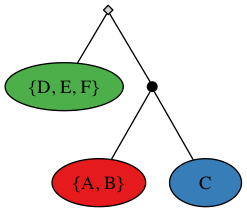
\includegraphics[max width=\linewidth]{fig/2/similar_tree1.png}
      \caption{$((\{AB\}, C), \{DEF\});$}
    \endminipage \hfill
    \minipage{0.5\textwidth}
      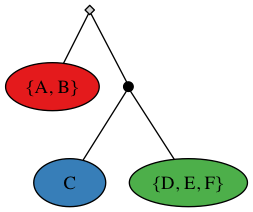
\includegraphics[max width=\linewidth]{fig/2/similar_tree2.png}
      \caption{$(\{AB\}, (C, \{DEF\}));$}
    \endminipage
  \end{figure}
  Закрашенный кружок обозначает предка, ромб обозначает здесь фиктивный корень.
\end{example}


На основе вышеизложенного сформулируем алгоритм \q{грубой силы}.
\begin{enumerate}
  \item Выделить среди статистик множество максимальных классов непересекающихся $\bb{C}$
  \item Отсортировать множество $\bb{C}$ по убыванию оценки
  \item Выбрать лучший по оценке класс
  \item Выделить разделения из статистик выбранного класса и собрать из них дерево
\end{enumerate}

\subsection{Реализация динамическим программированием}

Проблемой предыдущего алгоритма являлось то, что он выполнял перебор всех деревьев, о которых \q{свидетельствует} брейкпоинт-граф,
в случае многих геномов таких деревьев может быть много, что приведет к тому, что работа алгоритма может занять большое время.
Предположим, что для любой статистики $S$ с разделением вида $Q_1|Q_2$ из некоторого набора $\bb{S}$ известны поддеревья с наилучшей оценкой,
построенные на множествах геномов $Q_1$ и $Q_2$, тогда чтобы найти дерево с максимальной оценкой нужно перебрать все статистики из $\bb{S}$ и найти ту,
оценка которой в сумме с оценками поддеревьев даст наибольшее значение.
Данную логику можно применить также для того, чтобы построить оптимальные деревья для вышеупомянутых пар множеств $Q_1$ и $Q_2$,
составляющих разделения статистик.
Таким образом, приходим к задаче динамического программирования для решения которой сформулируем следующий алгоритм:
\begin{enumerate}
  \item Пусть для множества $F$ размера $f$, $size(F) = f$.
    Пусть даны множества $\bb{G}$ геномов и $\bb{S}$ имеющихся статистик.
    Введем структуру множеств $\{ SCLevel_i | i = 1..N \}$, где $N = size(\bb{G})$,
    при $\forall i, SCLevel_i$ - множество четверок вида $(C, V, V, ())$, таких что $size(C) = i$,
    $\exists S \in \bb{S}: (C = left(S) \vee C = right(S)) \wedge value(S) = V$,
    компоненты четверки обозначают соответственно: множество геномов, на котором построено дерево;
    оценку этого множества; суммарную оценку построенного дерева; пару множеств геномов, лежащих в левом и правом поддеревьях.
  \item Начиная с $i = 2$,
    $\forall c = (C, V, CS, SS) \in SCLevel_i$,
    $(C1, \_, CS1, \_) \in SCLevel_j$,
    $(C2, \_, CS2, \_) \in SCLevel_k$ обозначим, что $с = (C, V, V + CS1 + CS2, (C1, C2))$,
    если $V + CS1 + CS2$ - максимальное значение такое, что $j = 1..i-1$, $k = i - j$ и $C1 \cup C2 = C \wedge C1 \cap C2 = \varnothing$
  \item Пусть единственный элемент $SCLevel_N$ имеет вид $(\_, \_, \_, (C1, C2))$ тогда результирующее дерево можно построить сверху
    вниз для множеств $C1$ и $C2$, после чего объединить результаты корнем.
    Для множеств множеств $C1$ и $C2$ можно выполнить сборку тем же образом, базой для индуктивной сборки послужит случай,
    когда $C1$ и $C2$ - множества с одним элементом.
\end{enumerate}
